\chapter{Wall-function formulations and implementation}
\label{chap:wall-function-formulations}

The investigated wall functions combine momentum and thermal closures to infer wall shear stress and heat-flux from a sampled boundary layer state. Figure~\ref{fig:WF:wall-function-idea-illustration} shows this coupling: the sampled velocity and thermodynamic state, the physical wall temperature and the required reference information determine the wall loads. Their delivery to the CFD equations is distinct from the closure itself. Coupling to a RANS turbulence model additionally requires a compatible near-wall turbulence constraint.

\begin{figure}[H]
    \centering
    % Preserve the supplied raster diagram and typeset its wall label consistently.
    % Coordinates are relative to the 964 x 321 pixel source image.
    \begingroup
    \setlength{\unitlength}{\linewidth}
    \begin{picture}(1,0.33299)
        \put(0,0){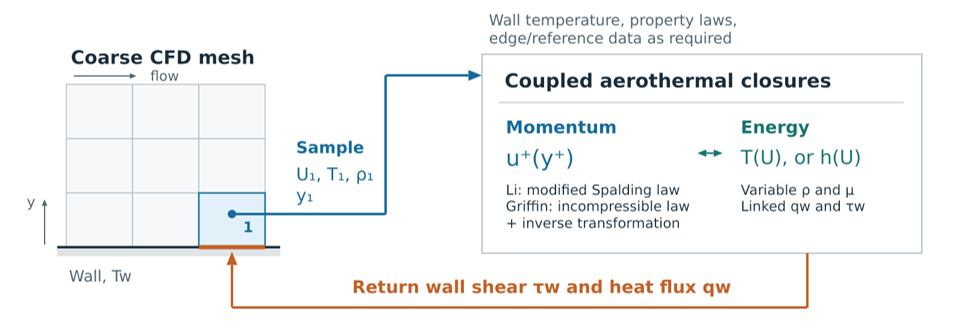
\includegraphics[width=\linewidth]{05_WF_Idea_Implementation/Wallfunction_Idea.png}}
        \put(0.0674,0.0342){\textcolor{white}{\rule{0.0778\unitlength}{0.0228\unitlength}}}
        \put(0.0716,0.0467){\makebox(0,0)[l]{\fontsize{8}{9.6}\selectfont\textcolor[RGB]{82,104,121}{Wall, \(T_w\)}}}
    \end{picture}
    \endgroup
    \caption{Wall-function coupling using the first cell as the sample. Momentum and thermal closures infer wall shear stress and heat-flux from the sampled state and the wall and reference conditions, and return these loads to the CFD solver.}
    \label{fig:WF:wall-function-idea-illustration}
\end{figure}

\section{Wall-function sampling and mesh geometry}
\label{subsec:wall-functions:sampling-geometry}

The wall-function sampling height is denoted by \(y_s\), and the wall-to-first-cell-centre distance by \(y_1\). On a conventional wall-function mesh, the first cell supplies the sample, so \(y_s=y_1\). Increasing the first-cell height consequently moves the sample outwards and coarsens the neighbouring internal-face stencils (Figure~\ref{fig:WF:wall-function-conventional-mesh}). The term \emph{conventional coarse wall-function mesh} refers to this coupled change in sampling height and mesh spacing throughout this work.

\begin{figure}[H]
    \centering
    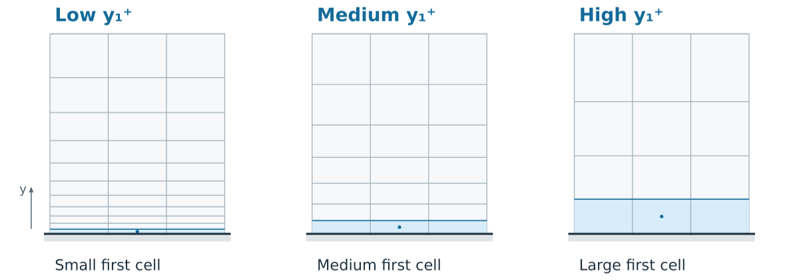
\includegraphics[width=\linewidth]{05_WF_Idea_Implementation/Wallfunction_Meshes.png}
    \caption{Conventional wall-function mesh strategy. Enlarging the wall-adjacent cell increases both the first-cell sampling height \(y_s=y_1\) and the spacing of the nearby internal-face stencils. The indicated wall-unit heights refer to the cell centres, not the full cell heights.}
    \label{fig:WF:wall-function-conventional-mesh}
\end{figure}

The implemented Li and Griffin wall functions can also sample an interior cell while retaining finer cells below it. The selected cell supplies the closure inputs and its wall-normal distance supplies \(y_s\), denoted \(y_m\) in Griffin's formulation. The associated SA constraint is applied at that same cell, while the predicted loads are delivered at the physical wall. The cells below the sample remain part of the CFD solution. This option separates closure sampling from the first-cell distance \(y_1\) and the centre separation \(h\) across an internal face at \(y_f\), defined in Equation~\eqref{eq:numerical-framework:internal-face-operators}. Because the wall loads are inferred from modelled wall slopes, the sample need not meet the wall-resolved secant requirement of Section~\ref{sec:openFOAM_qw_tauw}. Its location must nevertheless lie within the closure's applicable range. Moreover, prescribing the wall loads does not replace internal-face gradient reconstruction or transport-coefficient interpolation. Section~\ref{subsec:comparative:zpg:informed-mesh} uses the independent sampling option to assess the additional mesh requirement within the retained boundary layer. The following section first explains the common flux-delivery mechanism and subsequent sections present the individual closures and their RANS coupling.

\section{Wall-flux delivery in OpenFOAM/HiSA}
\label{sec:openFOAM_wall_function_implementation_general}

The standard wall-load evaluation in Section~\ref{sec:openFOAM_qw_tauw} combines a wall-to-cell gradient with an effective transport coefficient. Encoding a wall-function target through that coefficient is convenient, but constrains which loads can be delivered. This section motivates the direct wall-flux interface used for the investigated closures.

\subsection{Limitations of transport-coefficient boundary conditions}

A conventional implementation adjusts wall \texttt{nut} and \texttt{alphat} until the discrete gradient produces the target stress or heat-flux. For example, inversion of the planar-wall shear relation gives
\begin{equation}
    \nu_{t,w}
    =\frac{\tau_{w,\mathrm{target}}y_1}{\rho_w U_{1,t}}-\nu_w,
    \label{eq:nut_BC}
\end{equation}
where \(U_{1,t}>0\) denotes the tangential velocity magnitude. An analogous inversion determines the thermal coefficient from the target heat-flux and the wall-to-cell energy difference.

Requiring non-negative turbulent transport leaves the molecular contribution as the smallest representable flux magnitude for a given nonzero secant. It also fixes the flux direction to that of the secant. Neither condition is guaranteed to agree with a wall-function target. The thermal restriction is particularly relevant to non-monotonic temperature profiles: if a sample beyond the temperature maximum is colder than the wall while the physical wall remains cooled, a non-negative conductivity cannot deliver the required heat-flux through that wall-to-cell temperature difference. Even when the signs agree, the target can lie below the molecular secant contribution. These are limitations of the delivery mechanism, separate from closure accuracy.

\subsection{Limitations of a prescribed-gradient temperature condition}

A prescribed-gradient temperature condition can represent either heat-flux sign, but matching the target through the discrete gradient lets the patch temperature depart from the physical wall temperature used by the closure. On a coarse mesh, the resulting extrapolated face state can differ substantially from that physical state. Evaluating density and viscosity at this numerical face temperature then changes the wall transport properties and can make the molecular shear contribution exceed the target in Equation~\eqref{eq:nut_BC}. This approach therefore introduces an additional coupling between thermal flux delivery and momentum transport. Retaining the physical prescribed wall temperature while replacing the wall flux avoids this inconsistency.

\subsection{Direct wall-flux substitution}
\label{subsec:wall-functions:direct-flux-delivery}

% Implementation evidence:
% /home/mgnadlinger/OpenFOAM/mgnadlinger-v2412/modules/hysa/src/modules/hisa/wallFluxSubstitution.H
% /home/mgnadlinger/OpenFOAM/mgnadlinger-v2412/src/LiWallFunctions/DESIGN_AND_DEVIATIONS_LiFlux.md
% /home/mgnadlinger/OpenFOAM/mgnadlinger-v2412/src/GriffinWallFunctions/DESIGN_AND_DEVIATIONS_GriffinFlux.md
% Reporting verified against:
% /home/mgnadlinger/WF_validation/LowH_M3/validation/scripts/plot_wall_flux_sweeps.py
% /home/mgnadlinger/WF_validation/LowH_M3/validation/scripts/plot_opt_mesh_wall_flux_sweeps.py
The implemented interface replaces the explicit viscous wall-face contributions in HiSA's momentum and total-energy residuals. Each wall function publishes its target traction, target heat-flux and an active-face mask. HiSA first assembles the standard wall contributions, then adds the difference between the targets and those contributions on active faces. In a common convention, with traction acting on the fluid and heat-flux \(q_w\) positive into the wall, the corrections per unit area are
\begin{equation}
    \Delta\boldsymbol{\tau}
    =\boldsymbol{\tau}_{w,\mathrm{target}}-\boldsymbol{\tau}_{\mathrm{std}},
    \qquad
    \Delta q=-q_{w,\mathrm{target}}-q_{\mathrm{std}}.
    \label{eq:wall-functions:flux-substitution}
\end{equation}
The standard terms are the actual terms assembled by HiSA, including the full viscous traction and \(q_{\mathrm{std}}\) is positive into the fluid, following OpenFOAM's convention. The target traction is tangential, as assumed by the boundary layer wall closures. The energy correction includes the corresponding viscous work, which vanishes at a stationary no-slip wall. Inactive faces retain the standard evaluation.

For the isothermal cases, this interface keeps the physical fixed wall temperature and sets wall \texttt{nut} and \texttt{alphat} to zero; these fields no longer encode the target loads. The near-wall turbulence constraint remains a separate part of the RANS coupling. Direct substitution changes neither the wall-function closure nor the internal-face transport operators, and does not impose an exact off-wall profile. It removes the coefficient-inversion restriction while leaving closure error, turbulence-model error and spatial-discretization error to be assessed in Chapter~\ref{chap:comparative-evaluation}.

The imposed loads are recorded in the wall-function diagnostics. Li's native heat-flux is positive into the wall, whereas Griffin's and Wang's are positive into the fluid; the interface and comparison scripts convert these signs consistently. Standard \texttt{wallHeatFlux} and \texttt{wallShearStress} function objects do not include the residual correction and therefore do not report the imposed targets. The coupled wall-function comparisons use the diagnostic targets on active faces; the wall-resolved comparisons use the standard function-object output. The source code and case configurations are identified in the \hyperref[chap:data-avail]{data-availability statement}.

\section{Li wall function}
\label{sec:wall-functions:gao-li}

Li et al. developed an improved wall function for hypersonic reacting turbulent boundary layers, addressing strong wall cooling and variable gas properties~\cite{li2025WF}. Their comparison with the precursor formulation of Gao et al. shows substantially smaller skin-friction and heat-flux errors for the investigated cold-wall flat-plates~\cite[Section~IV.B, Figures~17--20]{li2025WF}. The improvements concern both the thermal relation and the treatment of variable properties in the velocity law. This motivates investigating the Li formulation here, while the earlier Gao formulation is not additionally being evaluated.

\subsection{Momentum and thermal closures}
\label{subsec:wall-functions:gao-li:governing-relations}

The thermal closure is a quadratic relation between static enthalpy and velocity~\cite[Eqs.~(12)--(15)]{li2025WF}. It extends the generalized temperature--velocity relation of Zhang et al. by using enthalpy to accommodate reacting-gas thermodynamics. Its generalized recovery enthalpy determines the wall slope and thereby relates heat-flux to wall shear, extending the fixed-recovery-factor prescription of the earlier Walz-based construction.
\par\medskip

The momentum closure combines a viscosity-corrected viscous-sublayer relation with a compressible logarithmic law in a unified expression~\cite[Eqs.~(27), (30)--(32)]{li2025WF}. It assumes approximately constant total shear stress in the inner layer and blends through the buffer layer. Sampling below the logarithmic region is therefore permitted by construction, although accuracy can still vary with sampling height.
\par\medskip

\label{subsec:wall-functions:gao-li:empirical-constants}
The formulation retains \(\kappa=0.41\) and \(B=6.0\) and approximates the viscosity variation by an enthalpy power law. Li et al. fit its exponent, denoted \(\omega_H\) here, to approximately \(0.72\) in their reacting viscous-sublayer profiles~\cite[Eq.~(25) and Figure~12]{li2025WF}. This transport approximation is calibrated for those conditions; its transfer to other gas models and wall temperatures is not automatically given and open to scrutiny.

\subsection{Non-reacting implementation and reference-state choice}
\label{subsec:wall-functions:gao-li:openfoam-implementation}

The present implementation uses fixed composition and omits chemical reactions and species-diffusion contributions. The enthalpy-based closure is retained. With the additional calorically perfect-gas assumption, \(h=c_pT\), its thermal relation reduces to the Zhang temperature--velocity relation reproduced by Li et al.~\cite[Eqs.~(8)--(13)]{li2025WF}. This equivalence concerns the thermal closure; the momentum closure remains Li's unified velocity law. Removing chemistry alone does not require constant specific heat.
\par\medskip

A useful feature is that the reference velocity and enthalpy need not be taken at the boundary layer edge. Li et al. reformulate both closures using an interior reference point and select the second off-wall grid point in their implementation~\cite[Section~IV.C, Eqs.~(40)--(42)]{li2025WF}. Here, the matching cell and a second cell farther from the wall provide the two velocity--enthalpy states. Together with the physical wall state, they determine the thermal relation. The unified velocity law is then inverted for the wall shear at the matching height, and the inferred thermal wall slope supplies the heat-flux. A prescribed-edge option is retained for comparison.
\par\medskip

This local reference construction avoids explicit edge detection, whose mesh-dependent reconstruction introduces additional sensitivity into Griffin's closure inputs (Section~\ref{subsec:wall-functions:griffin:edge-detection}). The second reference point remains distinct from the matching point; neither location should be confused with the full height of the wall-adjacent cell.
\par\medskip

\label{subsec:wall-functions:gao-li:turbulence-coupling}
The recovered shear stress and heat-flux are delivered directly to HiSA (Section~\ref{subsec:wall-functions:direct-flux-delivery}). Following Li et al.~\cite[Eqs.~(36)--(39)]{li2025WF}, the velocity-law derivative also supplies a compatible eddy viscosity and hence a constraint on the SA variable at the selected near-wall layer. This turbulence constraint is separate from prescribing the wall fluxes.

\subsection{Scope of the published assessment}
\label{subsec:wall-functions:gao-li:published-results}

The non-reacting flat-plate case in Li et al. checks the underlying solver and SA model against an experimental data and van Driest II theory~\cite[Section~IV.B and Figure~2]{li2025WF}. There it does not assess the improved wall function. The latter is tested on reacting flat-plates against resolved RANS solutions; the second-reference-point variant is demonstrated at first-point \(y^+=4\) and \(8\), whereas the coarser logarithmic-layer tests use edge quantities~\cite[Sections~IV.B--C]{li2025WF}. These results do not provide an independent DNS or experimental validation of the non-reacting wall function used here and can thus not be used as a way to validate the code implementation.
\par\medskip

Direct reproduction also requires care because Li et al. use a finite-difference solver. They define the wall distance to the first off-wall grid point, while their coupling acts on viscous fluxes between that point and the wall~\cite[Section~II.A, Eq.~(17) and Figure~16]{li2025WF}. Transfer to a finite-volume method requires matching the physical sampling and flux locations; equal reported \(y^+\) values alone do not establish an equivalent discretization. The published results therefore provide context rather than a direct verification case for the complete implementation.

\subsection{Reference sensitivity and assessment in this thesis}
\label{subsec:wall-functions:gao-li:limitations}

Avoiding edge detection does not remove all reference-state sensitivity. Inferring the thermal relation becomes poorly conditioned when the sampled and reference velocities nearly coincide, and both points must remain within the region represented by the closure. The prescribed-profile tests in Section~\ref{subsec:erriso:apriori-results} compare the second-point and prescribed-edge choices on the M6Tw025 DNS profile and the LowH\_M3 resolved SA profile. They show no systematic loss of accuracy from using the second point, supporting this practical advantage while retaining appreciable closure errors. These tests establish the standalone closure response before the coupled mesh sensitivity is examined in Section~\ref{subsec:comparative:zpg:yplus-sensitivity}.


\section{Griffin inverse-transformation wall function}
\label{sec:wall-functions:griffin}

Griffin et al. construct a compressible near-wall profile by applying an inverse velocity transformation to an incompressible wall law and closing the temperature profile through an algebraic temperature--velocity relation~\cite{griffin2022WFbrief,griffin2023WF}. The formulation accounts for density and viscosity variations associated with wall cooling while retaining a unified description of the viscous sublayer, buffer layer and logarithmic region. Its application here as a RANS wall function requires both the local matching state and information about the boundary layer edge.

\subsection{Momentum and thermal closures}
\label{subsec:wall-functions:griffin:governing-relations}

The momentum closure builds on the total-stress velocity transformation of Griffin et al.~\cite[Eqs.~(4)--(5)]{griffin2021Transformation}. It combines viscous scaling near the wall with turbulence-equilibrium scaling in the logarithmic region, blending between them through the buffer layer. The wall model uses its approximately constant-total-shear-stress form. Inverting this transformation converts the mean shear of a damped incompressible eddy-viscosity model into the compressible velocity gradient, including local density and viscosity variations~\cite[Eq.~(2.2)]{griffin2023WF}. The viscous limit recovers the linear wall law; the model is therefore not restricted by construction to logarithmic-layer sampling.
\par\medskip

The thermal closure is a quadratic temperature--velocity relation based on the generalized Reynolds analogy~\cite[Eq.~(2.5)]{griffin2023WF}. It satisfies the wall temperature and the sampled temperature at the matching velocity, while its wall slope is prescribed through the Reynolds analogy factor and the recovery temperature. The latter depends on the edge velocity and temperature. This wall slope links heat-flux directly to wall shear, without solving a separate temperature equation with an assumed constant turbulent Prandtl number. In Griffin's convention, heat-flux is positive into the fluid and negative for a cooled wall.
\par\medskip

For a prescribed wall temperature, the inputs are the velocity, temperature and density at the physical matching height \(y_m\), the edge state, an equation of state and a viscosity law. The inner reconstruction uses the ideal-gas law with approximately constant pressure and constant specific heat. A trial wall shear stress is used to integrate the inverse relation from the wall region to \(y_m\), updating temperature and transport properties along the reconstructed profile. The stress is iterated until the integrated velocity reproduces the sampled velocity; the thermal relation then supplies the heat-flux~\cite[Section~2.3]{griffin2023WF}. Both wall loads thus follow from reconstructed wall slopes rather than a wall-to-cell secant.
\par\medskip

The implementation retains the Reynolds-number-dependent calibration of the incompressible coefficients \(\kappa\) and \(A^+\) from the earlier research brief~\cite[Section~2]{griffin2022WFbrief}. These coefficients are selected using the edge-based semi-local friction Reynolds number, so the estimated thickness also enters the closure. The journal article examines this calibration but adopts fixed values \(\kappa=0.41\) and \(A^+=17\) for its subsequent simulations~\cite[Section~3]{griffin2023WF}. This distinction matters when comparing the implemented variant with published results.

\subsection{Boundary layer edge reconstruction and sensitivity}
\label{subsec:wall-functions:griffin:edge-detection}
\label{para:Griffin-BL-edge}

The edge quantities are obtained with Griffin et al.'s local-reconstruction method~\cite{griffin2021BLthickness}. It reconstructs a local inviscid velocity \(U_I\) from the stagnation enthalpy and identifies \(\delta_{99}\) where the actual tangential velocity first satisfies \(U/U_I=0.99\)~\cite[Eq.~(9) and Appendix~D, Eqs.~(D1)--(D2)]{griffin2021BLthickness}. This replaces comparison with a prescribed freestream velocity and permits a varying inviscid outer profile. The compressible construction assumes an inviscid, non-heat-conducting outer flow.
\par\medskip

In the present finite-volume implementation, cell-centre states are sampled outward from the wall, and their maximum stagnation enthalpy supplies the reconstruction reference. The first crossing of the squared velocity-ratio criterion brackets the edge. Its position, velocity and temperature are obtained by linear interpolation between the bracketing samples, using the squared ratio as interpolation coordinate. This interpolation is an implementation choice; the continuous edge criterion does not prescribe a discrete interpolation scheme.
\par\medskip

Figure~\ref{fig:wfs:BL_edge_quantities} illustrates the sensitivity for M6Tw025. The extracted thickness and edge temperature vary appreciably between conventional wall-function meshes, whereas the relative variation in edge velocity is smaller. These differences reflect both changes in the computed profiles and their discrete reconstruction; they do not isolate interpolation error. The two DNS markers further show that edge quantities must be compared using consistent definitions.
\par\medskip

These variations affect model inputs: edge velocity and temperature enter the thermal closure through the recovery temperature, and thickness enters the coefficient calibration described above. The physical matching height remains a separate input. The figure identifies an additional mesh dependence, but does not establish which edge quantity dominates the wall-flux error. This motivates separating the prescribed-profile closure tests in Section~\ref{sec:comparative:zpg:cross-comparison} from the coupled mesh assessment in Section~\ref{subsec:comparative:zpg:yplus-sensitivity}.

\begin{figure}[H]
    \centering
    % Figure provenance (WSL; absolute paths):
    %   Original export: /home/mgnadlinger/Xue_et_al/flat_plate/M6Tw025/validation/outputs_Griffin_SA/reported_edge_quantities.png
    %   Retained generator: /home/mgnadlinger/WF_validation/LowH_M3/Griffin_SA/analyze_griffin_edge_diagnostics.py
    %   Generator's original data root: /home/michael_gnadlinger/Xue_et_al/flat_plate/M6Tw025/WF/Griffin_SA
    %   Generator's original wall-resolved root: /home/michael_gnadlinger/TM_verification/SA/Zhang/M6Tw025_mesh_sens/5e-4_dx5
    %   Note: Retained export and generator checked; the exact companion CSV was not located.
    %   Note: The plotted DNS station is x=0.206771 m, distinct from the later matched comparison station.
    % End figure provenance.
    % Caption-sized typography (2026-10-19): 10 pt at 170 mm manuscript width.
    % Retained high-resolution curve pixels with vector labels and legend;
    % local source and audit: 05_WF_Idea_Implementation/griffin_edge_sources/.
    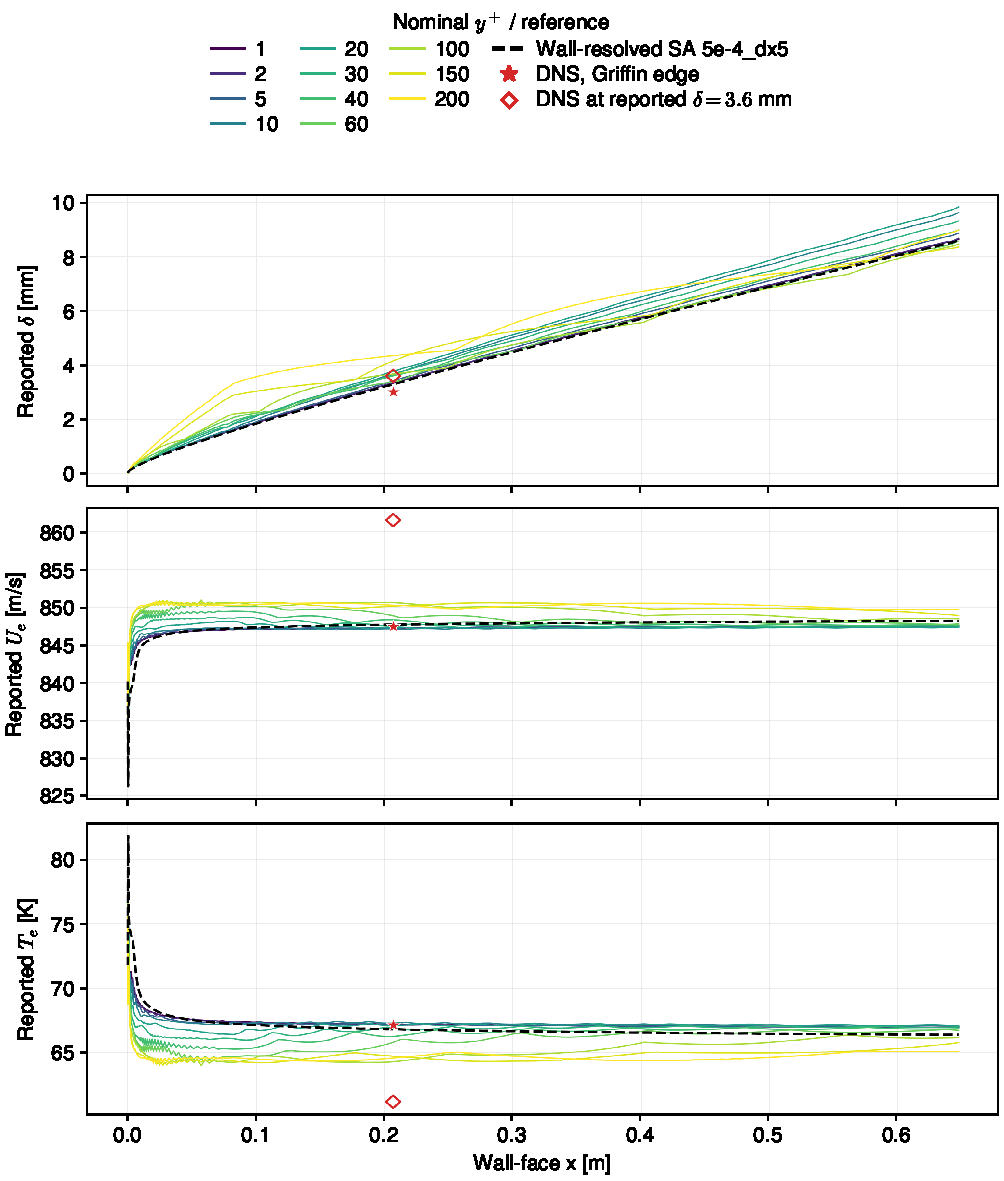
\includegraphics[width=\linewidth]{05_WF_Idea_Implementation/Griffin_Wallfunction_Edge_Quantities.pdf}
    \caption[Mesh sensitivity of the Griffin edge quantities]{Boundary layer thickness \(\delta\), edge velocity \(U_e\) and edge temperature \(T_e\) for M6Tw025. Colours identify conventional meshes by nominal first-cell \(y_1^+\); the dashed curve is the wall-resolved SA reference evaluated with the same criterion. Stars apply the Griffin criterion to the DNS profile, taking the unavailable mean wall-normal velocity as zero. Diamonds show the reported DNS thickness \(\delta=3.6\,\mathrm{mm}\) and the velocity and temperature interpolated at that height~\cite{zhang2018direct}.}
    \label{fig:wfs:BL_edge_quantities}
\end{figure}

\subsection{Application to RANS and limits of the published validation}
\label{subsec:wall-functions:griffin:validation-scope}

Griffin et al. describe the model as suitable for coupling to either LES or RANS. Their assessment combines a-priori tests on prescribed DNS profiles with a-posteriori WMLES of turbulent channels; it contains no coupled RANS validation~\cite[Sections~3--5]{griffin2023WF}. The principal comparisons use \(y_m=0.3\delta\), but the journal article also varies matching height during mesh refinement, including \(0.15\delta\) and \(0.075\delta\)~\cite[Section~4.1]{griffin2023WF}. These are matching locations, not prescribed first-cell-centre heights. As in WMLES it is common practice to retain off-wall resolutions below the point at which the wall model samples the boundary layer and then select the sample station adaptively dependant on the local boundary layer behaviour, i.e. if detachment is detected \cite{gao2026adaptive}. In addition to LES commonly using higher-order reconstruction methods, this may explain why Griffin et al. most likely didn't stumble upon  same mesh requirement issue (ref. Section \ref{subsec:comparative:zpg:yplus-sensitivity}).
\par\medskip

Here, the closure is coupled to SA through the near-wall turbulence constraint, with its wall shear and heat-flux delivered directly to HiSA as described in Section~\ref{subsec:wall-functions:direct-flux-delivery}. This RANS coupling and the reconstructed edge inputs require their own assessment. The published WMLES performance consequently provides no direct validation of the complete implementation. Nevertheless, the standalone closure can be checked against the published a-priori results, as shown in Table~\ref{tab:erriso:Griffin-a-priori-validation}. That consistency check supports the subsequent error-isolation study without implying equivalent accuracy of the coupled RANS calculations.

\section{Wang--Craft analytical wall function}
\label{sec:wall-functions:wang-craft}

The third an final wall function investigated in this work is by Wang et al \cite{wang2023WF}. It is unique compared Li et al and Griffin et al in that it does not rely on analytical momentum and energy closures, but rather on an analytical result of a proposed integral across the boundary layer. The downside of this approach being that it is not possible to run CFD independent analyses like the a-priori solves of the Li and Griffin wall functions (see Section~\ref{sec:comparative:zpg:cross-comparison}).
The implementation of this wall function raised several issue and ambiguities. Most notably on the streamwise integration necessary. While in the thesis work of Wang \cite{wang2019Thesis} it explicitly was implemented and tested on OpenFOAM there is no publicly available resource of the specific implementation. Contacting Wang unfortunately yielded in no response.
\par\medskip

The final implementation that was able to be achieved in the scope of this work showed some significant instabilities, most likely stemming from the downstream integration process at the leading edge of the flat-plates. Additionally the heat-flux and skin-friction output were unphysical. The afformentioned lack of a possibility to perform any kind of CFD-independent analysis further complicates debugging and identifying whether or not the issue is with the implementation or fundamentally with the wall function model - also because throughout the works of Wang on this wall function no investigation on a ZPG flat-plate was ever published. Thus it was decided to cut further debugging and development work in favour of spending the time on the analysis of the turbulence models and other two wall functions. 
\par\medskip

But for future research this wall function should anything but be disregarded, as it was the only investigated wall function that focused on, and proposed, good heat-flux and skin-friction prediction capability on SWBLI and complex geometries including separation.
